
%% ===============================================================================================
%% @author Leonardo Florez-Valencia (florez-l@javeriana.edu.co)
%% @author David Enrique Palacios García (david_palacios@javeriana.edu.co)
%% @author Karen Sofía Coral Godoy (corallg_ksofia@javeriana.edu.co)
%% ===============================================================================================

\documentclass[letter]{article}

\usepackage[spanish]{babel}
\usepackage[margin=1in]{geometry}
\usepackage{amsmath}
\usepackage{amsthm}
\usepackage{amssymb}
\usepackage[utf8]{inputenc}
\usepackage{graphicx, color}
\usepackage{algorithm}
\usepackage{algpseudocode}
\usepackage{mathrsfs}
\graphicspath{ {graphics/} }
% Some definitions
\floatname{algorithm}{Algoritmo}

% Author info
\title{Escritura del problema del camino más largo de vecinos en una matriz cuadrada}
\author{David Enrique Palacios García$^1$ \and Karen Sofia Coral Godoy$^1$}
\date{
	$^1$Departamento de Ingeniería de Sistemas, Pontificia Universidad Javeriana\\Bogotá,  Colombia \\
	\texttt{\{david\_palacios, corallg\_ksofia\}@javeriana.edu.co}\\~\\
	\today
}

\begin{document}
\maketitle
	
\begin{abstract}
En este documento se presenta la formalización del problema de encontrar el camino más largo de vecinos en una matriz cuadrada, junto con la descripción de un algoritmo de programación dinámica que lo soluciona. Además, se presenta un análisis experimental de este algoritmo.
\textbf{Palabras clave:} matriz, algoritmo, formalización, experimentación, programación dinámica.
\end{abstract}

\tableofcontents

	
\section{Introducción} \label{intro}
Encontrar los vecinos de cada posición de una matriz suena muy trivial, pues son aquellas casillas adyacentes a esta. Esto nos permite encontrar caminos entre las casillas, pues cada una de estas tiene a su vez más vecinos. No obstante, para este taller, únicamente nos interesan las casillas que contienen un valor numérico una unidad mayor que la casilla actual, lo que podría generar caminos basados en estos valores. Es así, como se plantea el objetivo de este taller: encontrar el camino más largo de vecinos en una matriz cuadrada, donde cada valor de la casilla es único y está determinado en el rango $[1,n]$, siendo $n$ el tamaño de la matriz cuadrada. Aquí, se busca solucionar el problema utilizando una estrategia de programación dinámica, con el objetivo de presentar: la formalización del problema (sección \ref{formalizacion}), la escritura formal del algoritmo (sección \ref{algoritmos}) y un análisis experimental del mismo (sección \ref{experimentos}).

\section{Formalización del problema} \label{formalizacion}
Cuando se piensa en {\it hallar los vecinos secuenciales de una casilla} la solución inmediata puede ser muy simplista: inocentemente, se piensa en tomar cada casilla y evaluar cuál de sus vecinos es mayor por una unidad. Sin embargo, con un poco más de reflexión, hay tres preguntas que pueden surgir:
\begin{enumerate}
  \item ¿Cuántos vecinos tiene cada casilla?
  \item ¿Existen vecinos diagonales?
  \item ¿Una unidad se refiere únicamente a números naturales?
\end{enumerate}

Para iniciar, recordemos que una matriz cuadrada $A$ cuya cardinalidad es mayor a 3, cuenta con casillas de ``centro``, esto es, que no son adyacentes al borde de la matriz. Si imaginamos un momento una casilla de este tipo, entenderemos que tiene 4 vecinos adyacentes. Aquellas que son esquinas, cuentan con 2 vecinos, y los que están al borde de la matriz, tienen con 3. Esto es importante porque hay que verificar qué tipo de casilla se está evaluando, para saber si es posible evaluar vecinos encima, debajo, a su izquierda o derecha.
Por lo que venimos hablando, vecinos diagonales no se tendrán en cuenta, únicamente verticales y horizontales. Para este problema, un vecino válido es aquel que tiene una unidad más que la casilla actual, por lo que únicamente se tendrán en cuenta números naturales entre $[1,n]$, siendo $n$ una de las dimensiones de la matriz cuadrada.

\subsection{Definición del problema de la ``multiplicación matricial''} \label{problema}
Así, el problema de encontrar la secuencia más larga de vecinos en una matriz cuadrada se define como
  \begin{enumerate}
    \item Una matriz cuadrada $A = \langle a_{1,1}, a_{1,2}, ... , a_{n,n}\rangle \in \mathbf{N^2} $ y existe una relación de igualdad y diferencia
    
    \item Entonces, el camino más largo de vecinos adyancentes de la casilla $A_{i,j}$ es: 
    
    \begin{equation}
        S_{i,j}= \left\{ \begin{array}{lcc}
             0 &   ;  & i < 1 \lor j < 1  \lor i > |A| \lor j > |A| \\
             \\ 
             max \left\{
             \begin{array}{lcc}
                  1 + S_{i-1,j}&  ;  & A_{i,j}+1 = A_{i-1,j} \land i>1   \\
                  \\
                 1 + S_{i+1,j}&  ;  & A_{i,j}+1 = A_{i+1,j} \land i<n   \\
                 \\
                  1 + S_{i,j-1}&  ;  & A_{i,j}+1 = A_{i,j-1} \land j>1   \\
                 \\
                 1 + S_{i,j+1}&  ;  & A_{i,j}+1 = A_{i,j+1} \land j<n   
                 
             \end{array}\right\} &  ; & otherwise
             \end{array}
   \right.
    \end{equation}
  \end{enumerate}



Producir una secuencia de números enteros $W$ que indique el camino más largo de vecinos adyacentes encontrado en una matriz cuadrada. 
\begin{itemize}
    \item Entradas:
    \begin{itemize}
        \item $A = \left< a_{1,1},a_{1,2}, ... , a_{n,n}\right> \in N^2 ~|~ a_{i,j} = v \in [1,n] $ y es único en $A$
    \end{itemize}
    \item Salidas:
    \begin{itemize}
        \item $W = \left< v \in A \right> ~ | ~ W ~ $ es una secuencia de números enteros que cumple la ecuación (1).
    \end{itemize}
\end{itemize}

\section{Algoritmo de solución} \label{algoritmos}

\newpage
\subsection{Programación dinámica- Backtracking}
\label{algoritmos:programaciondinamica}
La idea de este algoritmo es: encontrar la longitud del camino más largo de vecinos de cada una de las casillas de la matriz, para así determinar quienes hacen parte del mismo. Para evitar cálculos repetidos, se utiliza la matriz $M$, que guarda la mayor longitud calculada desde esa casilla. En cuestión del \textit{Backtracking}, se utiliza una matriz de duplas, donde se almacena la ubicación de la siguiente casilla del camino.

A pesar de que se sigue utilizando la recursión para hallar cada camino posible de cada casilla, la pila de ejecución no se llena porque únicamente se elige el vecino que cumple la restricción de ser una unidad mayor que la casilla actual. Al haber máximo un único valor que cumpla este requisito, no se evalúan todos los caminos sino el único que realmente es útil para resolver el ejercicio.

El resultado final quedará guardado en la casilla donde se tenga el mayor camino posible, creando a partir de allí el backtracking para encontrar la secuencia final.

\begin{algorithm}[!htb]
\caption{Calcular el camino más largo de la casilla i,j}
\begin{algorithmic}[1]
\Require {
$A = \left< a_{1,1},a_{1,2}, ... , a_{n,n}\right> \in N^2 ~|~ a_{i,j} = v \in [1,n] $ y es único en $A$
}
\Procedure{SecuenciaCrecienteAux}{$A,i,j,M,B$}
 \If{$i<1 \lor j<1 \lor i>|A| \lor j>|A|$}
 \State \textbf{return} 0
 \EndIf
 \If{$M[i][j] \neq 0$}
 \State \textbf{return} M[i][j]
 \EndIf
 
 \State{$q \leftarrow 1$}
 \State{$sup,inf,izq,der \leftarrow 0$}
 
 \If{$i>1$}
    \If{$A[i][j]+1=A[i-1][j]$}
    \State{$sup \leftarrow 1 + \Call{SecuenciaCrecienteAux}{A,i-1,j,M,B} $}
    \State{$B[i][j] \leftarrow (i-1,j)$}
    \EndIf
 \EndIf
 
 \If{$i<|A|$}
    \If{$A[i][j]+1=A[i+1][j]$}
    \State{$inf \leftarrow 1 + \Call{SecuenciaCrecienteAux}{A,i+1,j,M,B} $}
    \State{$B[i][j] \leftarrow (i+1,j)$}
    \EndIf
 \EndIf
 
 \If{$j>1$}
    \If{$A[i][j]+1=A[i][j-1]$}
    \State{$izq \leftarrow 1 + \Call{SecuenciaCrecienteAux}{A,i,j-1,M,B} $}
    \State{$B[i][j] \leftarrow (i,j-1)$}
    \EndIf
 \EndIf
 
 \If{$j<|A|$}
    \If{$A[i][j]+1=A[i][j+1]$}
    \State{$der \leftarrow 1 + \Call{SecuenciaCrecienteAux}{A,i,j+1,M,B} $}
    \State{$B[i][j] \leftarrow (i,j+1)$}
    \EndIf
 \EndIf

 \State{$q\leftarrow \Call{max}{q,sup,inf,izq,der}$}
 \State{$M[i][j]\leftarrow q$}
      
\State \textbf{return} $M[i][j]$
\EndProcedure
\end{algorithmic}
\end{algorithm}

\begin{algorithm}[!htb]
\caption{Obtener secuencia creciente de vecinos en matriz cuadrada}
\begin{algorithmic}[1]
\Require {
$A = \left< a_{1,1},a_{1,2}, ... , a_{n,n}\right> \in N^2 ~|~ a_{i,j} = v \in [1,n] $ y es único en $A$
}
\Procedure{SecuenciaCrecienteEnMatriz}{$A$}
\State{$M \leftarrow ~ Matrix(A.row,A.row,unsigned~int)={0}$ }
\State{$B \leftarrow Matrix(A.row, A.row, Pair(A.row, (1,1))$}
\State{$q \leftarrow 1$}

\For{$i \leftarrow 1~\mathbf{to}~|A|~\mathbf{step}~1$}
    \For{$j \leftarrow 1~\mathbf{to}~|A|~\mathbf{step}~1$}
        \State{$B[i][j] \leftarrow (i,j)$}
    \EndFor
\EndFor

\State{$posActual \leftarrow (1,1)$}

\For{$i \leftarrow 1~\mathbf{to}~|A|~\mathbf{step}~1$}
    \For{$j \leftarrow 0~\mathbf{to}~|A|~\mathbf{step}~1$}
        \State{$k \leftarrow \Call{SecuenciaCrecienteAux}{A,i,j,M,B}$}
        \State{$q \leftarrow \Call{max}{q,k}$}
        \If{$q = M[i][j]$}
            \State{$posActual \leftarrow (i,j)$}
        \EndIf
    \EndFor
\EndFor

\State{$P \leftarrow \Call{List}{unsigned ~ int }$}

\While{$posActual \neq B[posActual.first][posActual.second]$}
\State{$\Call{append}{P,A[posActual.first][posActual.second]}$}

\State{$posActual \leftarrow B[posActual.first][posActual.second]$}
\EndWhile

\State{\Call{append}{$P,A[posActual.first][posActual.second]$}}

\State \textbf{return} $P$

\EndProcedure
\end{algorithmic}
\end{algorithm}


\newpage

\subsubsection{Análisis de complejidad} \label{algoritmos:inocente:complejidad}

Por inspección de código: Se puede observar que, el algoritmo más complejo es \texttt{$SecuenciaCrecienteEnMatriz$}, con 2 ciclos anidados. Lo cierto es que por la naturaleza de la programación dinámica, se ahorran cálculos repetidos, por lo que se acelera el proceso y se busca evitar llenar la pila de ejecución del procesador. Esto resulta en una complejidad de $O(n^2)$, siendo esta una expresión cuadrada. A pesar de que la solución es un poco demorada, se debe a la complejidad del problema en sí, puesto que se necesitan calcular todos los posibles caminos de cada uno de las casillas de la matriz.

\subsubsection{Invariante} \label{algoritmos:inocente:invariante}

La invariante al igual que la de todos los algortimos de programación dinámica es que se asegura que la tabla en cada iteración se esta completando correctamente.

\section{Análisis experimental} \label{experimentos}

En esta sección se presentarán los resultados del experimento para confirmar el orden de complejidad de los algoritmos presentados en la sección \ref{algoritmos} y la precisión de la solución. 

\newpage

\subsection{10 tamaños de matrices} \label{experimentos:aleatorias}

Acá se presentan los experimentos cuando el algoritmo se ejecuta tomando como párametro de entrada, números de matrices diferentes para cada iteración.

\subsubsection{Protocolo}
\begin{enumerate}
    \item Definir una muestra de 10 tamaños de matrices
    \item El algoritmo se ejecutará 10 veces con un parámetro de entrada diferente entre 2 y 100, que representa el tamaño de la matriz de cada iteración.
    \item Se genera el gráfico necesario para realizar un análisis.
\end{enumerate}

\subsubsection{Experimentación}
\begin{enumerate}
    \item Se utilizó el programa \texttt{$run\_random\_experiment$} al cual le llega como parámetro un $n$ de la muestra de 10 números que corresponden al tamaño de la matriz que se contempla en cada iteración del experimento, estos son:
    \begin{itemize}
        \item \texttt{2,12,22,32,42,52,62,72,82,92} 
    \end{itemize}

Adicionalmente, el programa teniendo en cuenta el tamaño de la matriz, completa internamente el contenido de esta de forma aleatoria cumpliendo con las restricciones definidas en secciones anteriores.
    
    \item El programa logró finalizar sin complicaciones con todos los tamaños de matrices propuestos, el tiempo empleado en cada iteración se registra en la siguiente tabla: (ver Tabla 1).
    
    \begin{figure}[h]
    \centering
    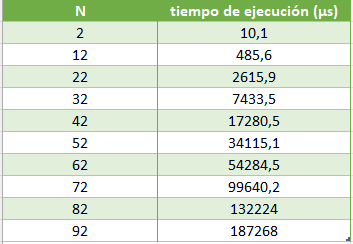
\includegraphics[scale=1]{Data.png}
    \label{experimentos:aleatorias:grafica}
     \caption{DataExperiment}
\end{figure}
    
    \item Se obtuvo las 10 secuencias crecientes de cada matriz cuadrada planteada con el tiempo de ejecución que se empleo para llegar a dicha solución, logrando así crear la siguiente gráfica: (ver Figura 1)
    
    \newpage
    
   \begin{figure}[h]
    \centering
    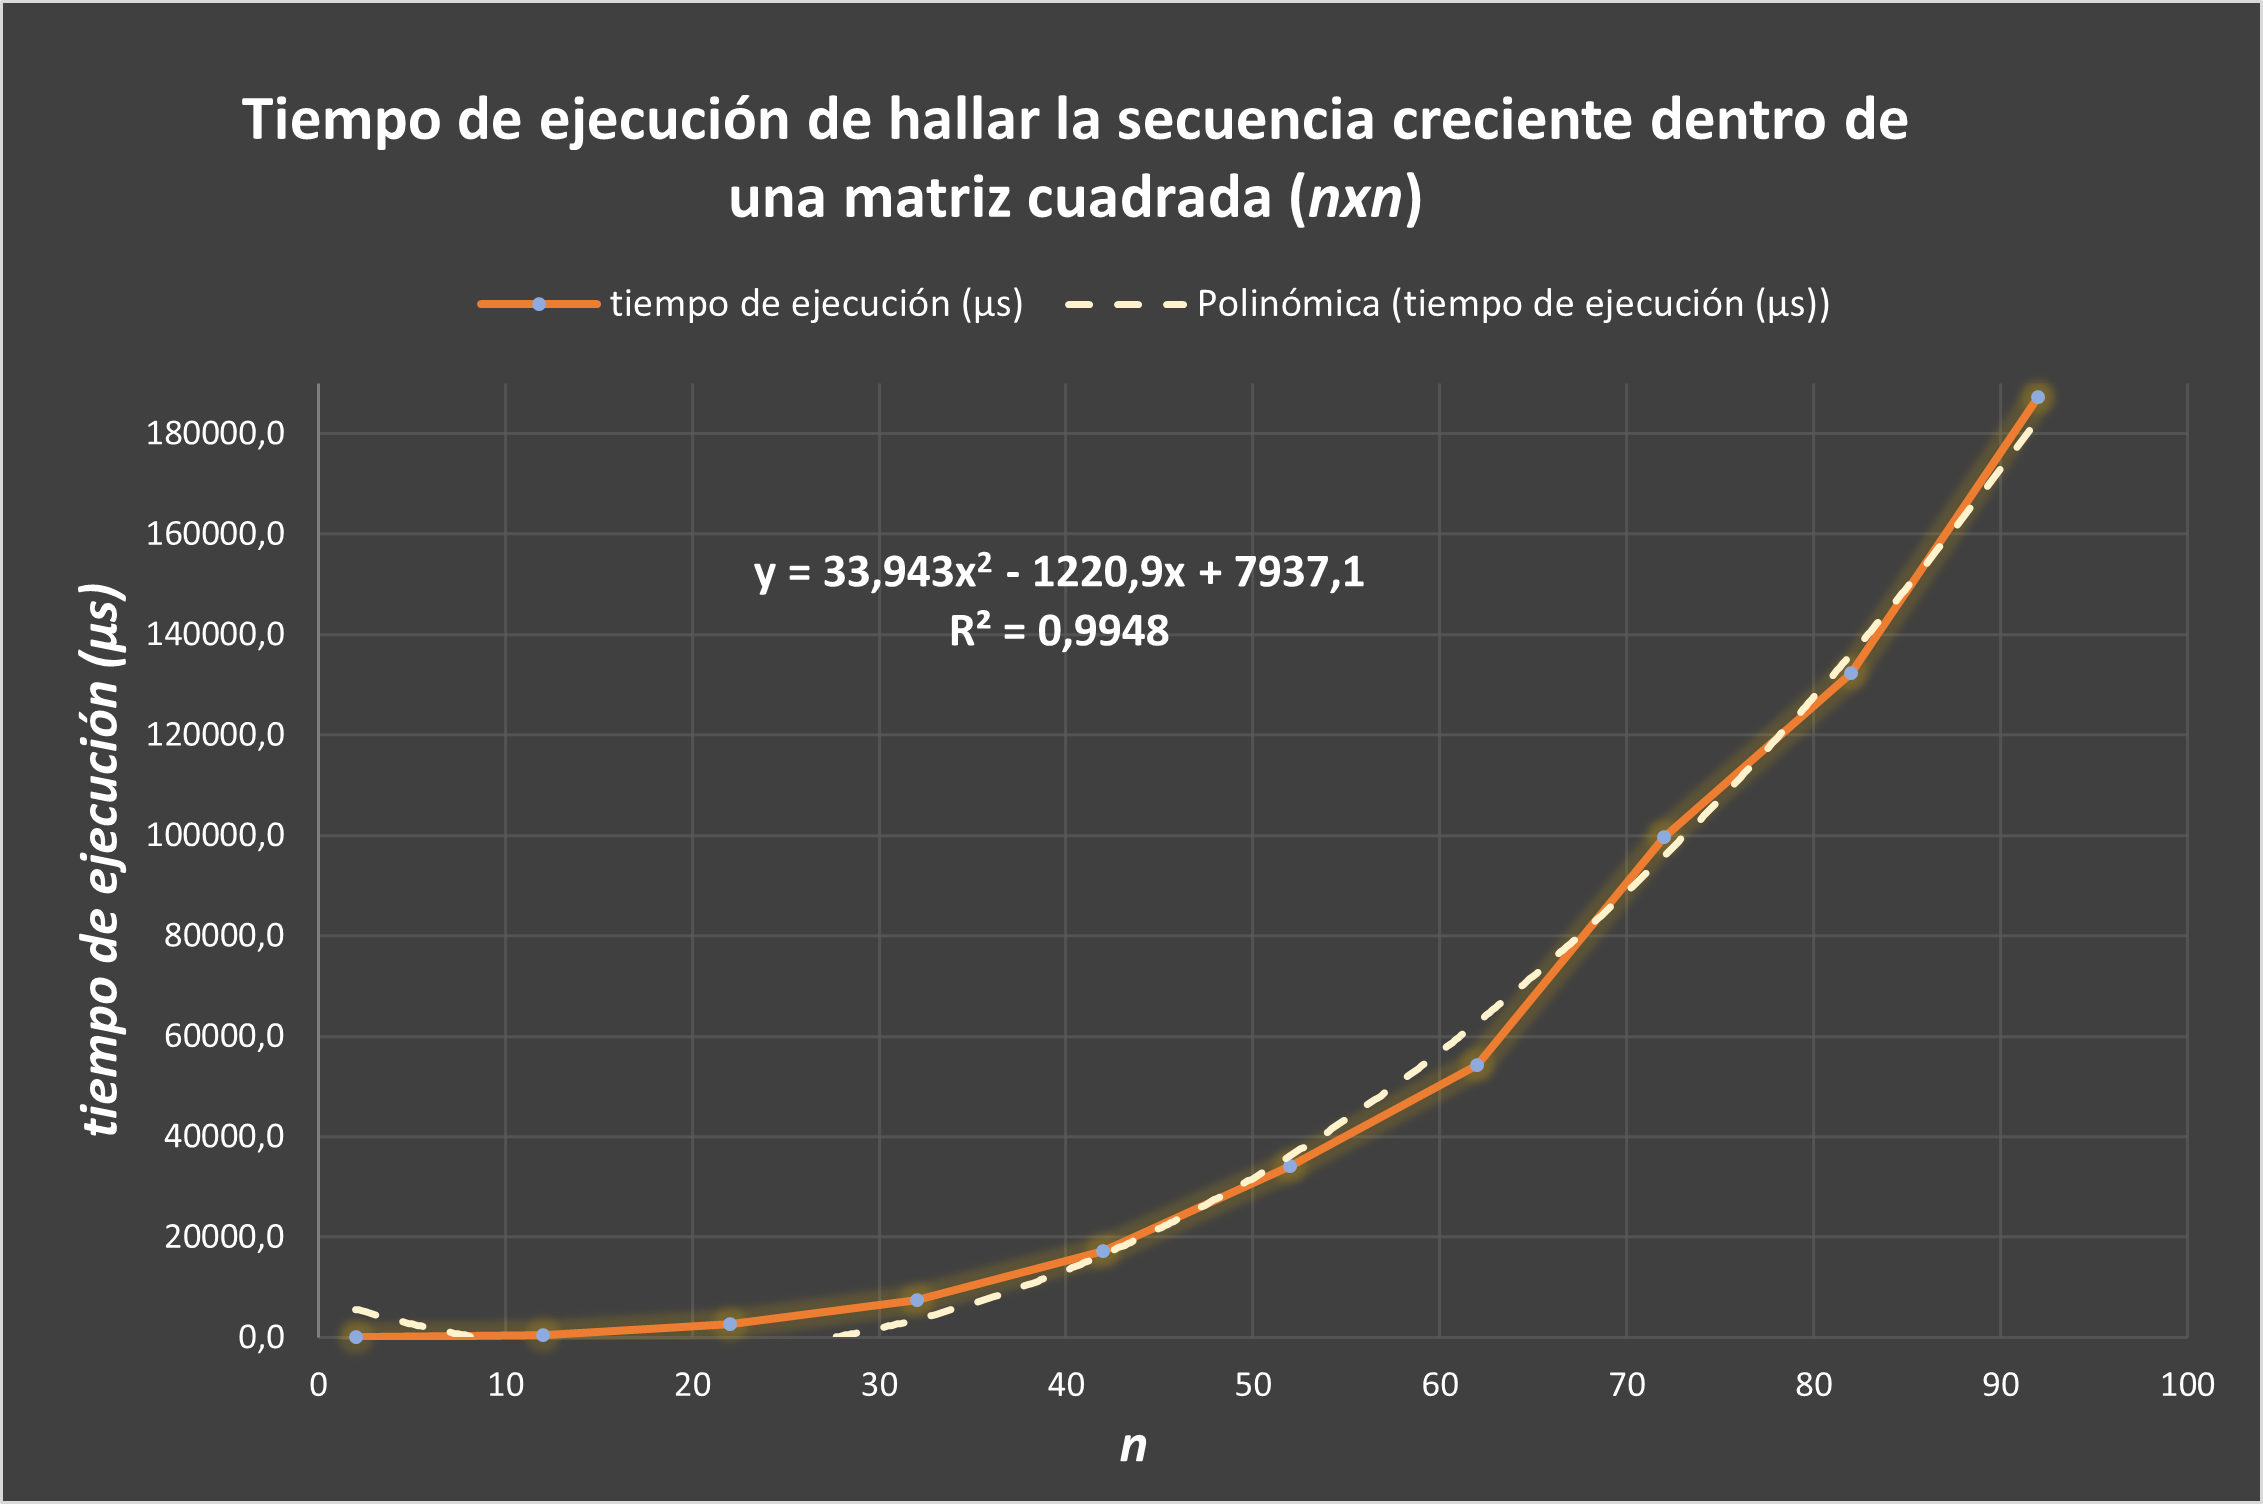
\includegraphics[scale=0.9]{DataGraphic.png}
    \label{experimentos:aleatorias:grafica}
    \caption{Tiempo de ejecución del algoritmo respecto a las dimensiones de la matriz}
\end{figure} 
    
\end{enumerate}



\subsubsection{Análisis del experimento}
\label{experimentos:aleatorias:analisis}
Como se expresó previamente, el algoritmo expuesto tiene una complejidad de $O(n^{2})$, sin embargo, en términos de tiempo de ejecución, es un proceso que llega a tomar mucho más tiempo cuando las dimensiones de la matriz es mayor. Esto pudo confirmarse, utilizando herramientas de Microsoft Excel, en donde se aplicó una regresión polinomial, hallando la línea de tendencia del algoritmo, su ecuación y valor $R^{2}$ que estaba muy cercano a 1, lo cual indica que se empleó el modelo más preciso, y por ende se reafirma la complejidad algorítmica de la solución presentada.  \\

Por otro lado, para este experimento, se realizó la una prueba de escritorio de la iteración con $n$ más pequeño para poder tener una comparación o evaluación del algoritmo. Los resultados se expresan a continuación: 

\begin{itemize}
        \item \texttt{Iteración: 1} 
        \item \texttt{Tamaño de la matriz: 2x2}
        
        \item 
        \texttt{A: }
        
        \begin{figure}[h]
  
    \includegraphics[scale=1]{matriz.png}
    \label{experimentos:aleatorias:grafica}
\end{figure}
    
        \item
        \texttt{Solución- : : [1, 2, 3, 4] }
    \end{itemize}
    
Con esta iteración se puede validar que el algoritmo funciona, ya que se hallo la secuencia creciente de mayor longitud teniendo en cuenta las restricciones del diseño del algoritmo.

\section{Conclusiones}
El experimento fue útil para concluir:
\begin{enumerate}
    \item Al aumentar las dimensiones de la matriz y por ende la cantidad de elementos de esta, los caminos que debe evaluar y el tiempo de ejecución también aumentan.
    \item Para plantear una solución de programación dinámica es importante considerar los parámetros de entrada, como en el caso de hallar la secuencia creciente más larga dentro de una matriz cuadrada  en donde, posiblemente usar un algoritmo inocente llenaria la pila de ejecución al experimentar con entradas de valores grandes.
    \item La programación dinámica se puede aplicar en los problemas de optimización ya que se basa en la idea de recursividad. En esta, se resuelven problemas descomponiéndolos en subproblemas similares más pequeños y usando dichas soluciones parciales de los subproblemas para llegar a una respuesta final. Cada subproblema se resuelve sólo una vez y su resultado es almacenado, evitando el trabajo de recalcular cada vez que el subproblema es nuevamente encontrado.

    \item En general, el tiempo de un algoritmo de programación dinámica depende del número de subproblemas y del número de opciones a revisar para cada subproblema.
\end{enumerate}
\end{document}

%% eof - sorting.tex
